\documentclass[../main.tex]{subfiles}
\begin{document}
\setchapterstyle{kao}
\setchapterpreamble[u]{\margintoc}
\chapter[Differential forms II]{Differential forms II\footnotemark[0]}
\labch{diff_form_II}
\section*{Settings}
Our starting point will be a differentiable manifold $\mathbf{M}$, at some point we will have some local charts $A=\{(u_{\alpha},\varphi_{\alpha})\}_{\alpha\in A}$. What is relevant for us is that our manifold has a tangent space for every point, so we can assign a 1-form, or more generally a k-form, on each of these linear spaces. If we do it in a smooth way, we will have a differential form. 
\begin{figure}[H]
	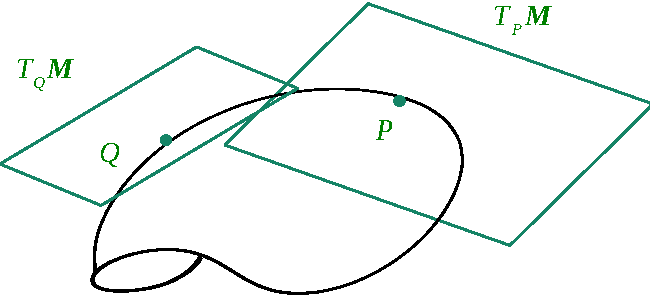
\includegraphics{images/differential_forms_scheme_II.pdf}
	\caption{Scheme of the tangent spaces in the points $P,M\in\mathbf{M}$.}
	\labfig{diff-forms-scheme-II}
\end{figure}
The prototype is the definition of vector field:\marginnote[5mm]{This definition would have been more appropriate in \refch{tang_space}.}
\begin{definition}[Vector field]\index{Vector field}
A vector field is a map
\[\mathbf{M}\ni {\color{red}p}\mapsto v\in T_{\color{red}p} \mathbf{M} \ \textrm{ s. t. the correspondence is smooth}\]
i.e. such that for \textbf{\underline{some}} [and, hence, for \textbf{any}] local chart $(u,\varphi)$ the local decomposition on the coordinate basis $V=\sum_{j=1}^n v^j(p)(e_j)_p$\marginnote{Also the local basis depends on the point, if you change the point the basis changes. We will not be pedantic on this notation, although \cite{doCarmo1994} uses the pedantic one $(e_j)_p$.} provides $\mathbf{C^{\infty}}$\textbf{-smooth functions} $\mathbf{M}\ni p\mapsto v^j(p)\in\mathbb{R}$.
\end{definition}
% 1:30:04
The trick is that we want to define a vector field as an assignment of a vector in every tangent space which is smooth. but we are not allowed to say that is smooth by using the ambient space\sidenote{Because there is no ambient space} and so the trick is to specify that in some chart the components will be smooth. If we change our chart, the components will change, but the smoothness will be preserved, because the change of coordinates is a smooth diffeomorphism and smoothness goes into smoothness. Therefore we have to check it just in one chart to be automatically true in every other chart. Differential 1-forms are similar to a vector field, but instead they use a covector, so they could be referred as covector fields:
\begin{definition}[(Differential) 1-form]\index{Differential 1-form}
A differential 1-form is a map $\alpha$
\[
\mathbf{M}\ni{\color{red}p}\mapsto \alpha_{\color{red}p}\in\Lambda^1 T_{\color{red}p}\mathbf{M}=T_{\color{red}p}^*\mathbf{M}\]
such that for some (and, hence, for any) local chart $(u,\varphi)$ the components with respect to the \textbf{dual basis}\marginnote{The dual bases depends, of course, on the chart.} $\{dx^1,\dots,dx^n\}$ are smooth, i.e. $\alpha=\sum_{j=1}^n\alpha_j(p)(dx^j)_p$ provides $\mathbf{C^{\infty}}$\textbf{-smooth functions} $\mathbf{M}\ni p \mapsto \alpha_j(p)\in\mathbb{R}$.
\end{definition}

\begin{definition}[Differential k-form]\index{Differential k-form}
A differential k-form is a map $\omega$\marginnote{In \cite{doCarmo1994} there is a $\ast$ ($T_P^\ast$), but it should be a typo.} \[\mathbf{M}\ni p\mapsto\omega\in\Lambda^k T_p\mathbf{M}\] such that for some (and, hence, for any) local chart, the components are $\mathbf{C^{\infty}}$\textbf{-smooth}.
\end{definition}

\section{Wedge product of a differential form}
We inherit everything from the linear theory in $E\cong\mathbb{R}^n$. In the following, we will denote with $\Omega^k(\mathbf{M})$ the space of k-differential forms, which is a \textbf{linear space}.

\begin{definition}[Wedge product of a differential form]\index{Wedge product of a differential form}
Let $\omega\in\Omega^k(\mathbf{M})$ and $\eta\in\Omega^l(\mathbf{M})$.
\[
(\omega\wedge\eta)_{\color{red}p}:=\omega_{\color{red}p}\underset{\mathclap{\tikz \node {$\uparrow$} node [below=1ex] {\footnotesize Wedge product in $T_p\mathbf{M}\cong\mathbf{R}^n$ };}}\wedge\eta_{\color{red}p}
\]
\end{definition}

\underline{Rem:} One always has to check that $p\mapsto(\omega\wedge\eta)_p$ is still $\mathbf{C}^{\infty}$\textbf{-smooth}. You can do it in a local chart .

\section{Exterior derivative (\href{https://it.wikipedia.org/wiki/\%C3\%89lie_Joseph_Cartan}{Cartan})}\marginnote{"\href{https://it.wikipedia.org/wiki/Derivata_esterna}{Derivata esterna}" in Italian.}
For convenience, we define the 0-forms as (smooth) functions, so the space $\Omega^0(\mathbf{M})$ corresponds to $\mathbf{C}^{\infty}(\mathbf{M})$. The idea of Cartan was to build an universal differential, which is intrinsic, i.e. it does not depend on the local coordinates:

\[
\Omega^0(\mathbf{M})\xrightarrow[]{\textrm{d}}\Omega^1(\mathbf{M})\xrightarrow[]{\textrm{\textrm{d}}}\Omega^2(\mathbf{M})\xrightarrow[]{\textrm{d}}\Omega^3(\mathbf{M})
\]

$\textrm{d}$ must be compatible with the \textbf{linear structure}, with the \textbf{wedge product}\sidenote{We would like to have it Leibnitz, but actually is impossible. It is Leibnitz up to a sign.} and with the fact that:

\[
\begin{split}
\Omega^0(\mathbf{M}) & \xrightarrow[]{\textrm{d}} \Omega^1(\mathbf{M})\\
f &\mapsto \textrm{d}f
\end{split}
\]

$\textrm{d}f$ should be the usual differential of a function $f:\mathbf{M}\xrightarrow[]{\mathbf{C}^{\infty}}\mathbb{R}$ (\refch{tang_space}), i.e.
\[
\textrm{d}f_p: T_p\mathbf{M}\xrightarrow[]{}\mathbb{R} \ \textrm{with} \ \textrm{d}f_p\in T_p^*\mathbf{M} \quad  \text{\parbox{3 cm}{\centering linear 1-form \\[-4pt]  at every point}}
\]
defined as:
\[
\textrm{d}f_p([\gamma])=\frac{\textrm{d}}{\textrm{d}t}(f\circ\gamma)(t)\big|_{t=0}\overset{\textrm{L.C.}}{=}\sum_j\frac{\partial f}{\partial x^j}\left(x(\gamma(0))\right)v^j
\]


\begin{theorem}[E. Cartan]
There exists a unique\footnote{And therefore it is an intrinsic object.} map $\textrm{d}:\Omega^k(\mathbf{M})\xrightarrow[]{}\Omega^{k+1}(\mathbf{M})$ such that:
\begin{enumerate}
    \item $\textrm{d}$ is \textbf{linear}
    \item $\textrm{d}$ is \textbf{pseudo-Leibnitz}: $d(\omega\wedge\eta)=d\omega\wedge\eta{\color{red}+(-1)^{\text{\textrm{deg}}\omega}}\omega\wedge d\eta\\ \forall\omega\in\Omega^k(\mathbf{M}),\eta\in\Omega^l(\mathbf{M})$
    \item if $\phi\in\Omega^0(\mathbf{M})=\mathbf{C^{\infty}(\mathbf{M})}$, then $\textrm{d}\phi$ is the ordinary differential (see above);
    \item $\textrm{d}^2=0:\forall\omega\in\Omega^k(\mathbf{M})$ one has $d({\color{red}d\underset{\mathclap{\tikz \node {$\uparrow$} node [below=1ex] {\footnotesize (k+1)-form };}}\omega})=0$.
\end{enumerate}
\end{theorem}
We never introduced one, but in a local chart, if $\omega\in\Omega^k(\mathbf{M})$ has local expression $\omega=\sum\omega_I(x)\textrm{d}x^I$, \marginnote{With $I$ we denote the set $(i_1,\dots,i_k)$ such that $i_1<\dots<i_k$ and with $dx^I$ we denote $dx^{i_1}\wedge\dots\wedge dx^{i_k}$} then $\textrm{d}\omega$ can be written as
\[
\textrm{d}\omega=\sum(\textrm{d}\omega_I(x))\wedge dx^I \qquad \Big|\Big| \star
\]
\begin{proof}
See \sidecite{von1978differential} omitted here.
\end{proof}
%INIZIO LEZIONE 7 - 24/03/2022
\begin{kaobox}[frametitle=Remark]
The "opposite2 approach is also possible. One might define the exterior differential via ($\star$), and then prove that it satisfies properties (1)-(4) and it is \textbf{intrinsic} (i.e. independent of the choice of a chart).
\end{kaobox}
\begin{kaobox}[frametitle=Remark]
There exists also the \textbf{ie derivative} of a differential form $\omega\in\Omega^k(\mathbf{M})$ along a vector field $V\in\nu(\mathbf{M})$ denoted by
\[
\mathcal{L}_V\omega
\]
This topic will not be covered here\footnote{But it is covered in Capitolo 8 of \cite{ferrari2020general}.}.
\end{kaobox}
\subsection{Examples}
For a physics what is important is to learn how to use the exterior differential, so we now see some examples.\\
\paragraph{$\boxed{k=0}$}Let $\phi\in \Omega^0(\mathbf{M}=C^\infty(\mathbf{M})$
\[
\textrm{d}\phi(V) \overset{\textrm{L.C.}}{=}\sum\frac{\partial\phi}{\partial x^j}(x)v^j
\]
Because $v^j=dx^j(V)$. one can also write
\[
\textrm{d}\phi=\sum_j\frac{\partial\phi}{\partial x^j}(x)dx^j
\]
Let us notice that it has the same information of the gradient, but with a little important difference. the differential applied to $V$ is intrinsic. I fyou want to wirte as a matrix it should be written like
\[
\textrm{d}\phi(V)=\underbrace{\left(\frac{\partial \phi}{\partial x^1}, \dots, \frac{\partial \phi}{\partial x^n}\right)}_{covariant}
\overbrace{
\begin{pmatrix}
v^1\\
\vdots\\
v^n
\end{pmatrix}
}^{\textrm{contravariant}}
\]
If we change local chart, both of them will change according to the Jacobian matrix of the transformation, but they will change the opposite way and the two Jacobian matrix will cancel each other $JJ^{-1}$, leaving the same intrinsic object. Contrast to the \textbf{gradient}\index{Gradient}, which is a vector, whose j component is the j-derivative\sidenote{If we use the Ricci's rule we see immediately that something is wrong with the index, this is because we need to put a metric.} 
\[
\left(\grad \phi\right)^j(x)=\sum_l\delta^{il}\frac{\partial\phi}{\partial x^l}(x)
\]
The information they contain is the same, but the first is much more natural when we change coordinates.
\paragraph{$\boxed{k=1}$} Suppose we have a one form
\[
\alpha \in \Omega^1(\mathbf{M} \qquad \alpha = \sum_j A_j(x)dx^j
\]
Let us differenciate $\alpha$
\[
\begin{split}
\textrm{d}\alpha
&=\sum_j\left({\color{red} \textrm{d}}A_j(x)\right){\color{red}\wedge}dx^j=\\
&=\sum_j\sum_l\frac{\partial A_j}{\partial x^j}(x)dx^l{\color{red}\wedge}dx^j=\\
&=\sum_{\color{red}l<j}\frac{\partial A_j}{\partial x^j}(x)dx^l\wedge dx^j+\sum_{\color{red}l\geq j}\frac{\partial A_j}{\partial x^j}(x)dx^l\wedge dx^j
\end{split}
\]
notice that $dx^l\wedge dx^j=0$ ($\alpha \wedge\alpha=0$ \textbf{always!}) and moreover that $x^2\wedge dx^1={\color{red}-}x^1\wedge dx^2$. So we can reorder the indices in the second sum and obtain\marginnote{The final formula is without the green comment.}
\[
\textrm{d}\alpha=\sum_{\color{red}l<j}\underbrace{\left(\frac{\partial A_j}{\partial x^j}(x){\color{red}-}\frac{\partial A_j}{\partial x^j}(x)\right)}_{\color{teal} \left(\textrm{rot}\Vec{A}\right)_{lj}}dx^l\wedge dx^j
\]
This is something failiar, identifying $\alpha$ with a vector field (neglecting that the indices are downstairs)
\[
\alpha = \sum_j A_jdx^j \ \longleftrightarrow \ \Vec{A}=\left(A_1,A_2,A_3\right)
\]
\paragraph{$\boxed{k=2}$} Suppose to have
\[
\eta \in \Omega^2(\mathbf{M}) \quad \eta = \sum_{i<j} \eta_{ij}(x)dx^i\wedge dx^j
\]
We can differenciate applying the rule
\[
\begin{split}
\textrm{d}\eta
&=\sum_{i<j}\left({\color{red} \textrm{d}}\eta_{ij}(x)\right){\color{red}\wedge}dx^i\wedge dx^j=\\
&=\sum_{i<j}\sum_l\frac{\partial \eta_{ij}(x)}{\partial x^j}dx^l{\color{red}\wedge}dx^i\wedge dx^j=\\
&=\textrm{reorder}=\\
&=\sum_{l<i<j}\big(\quad\Big)dx^l<dx^i\wedge dx^j
\end{split}
\]
Explicitly, for the case in which the dimension of the manifold is $n=\textrm{dim}\mathbf{M}=3$ one has\marginnote{It is usual to take a different bases. We want to identify them with thecanonical bases, but this works only in $\mathbb{R}^3$}
\[
\eta=P(x)\underbrace{dx^2\wedge dx^3}_{\color{teal} e_1}+Q(x)\underbrace{dx^3\wedge dx^1}_{\color{teal} e_3\wedge e_1 = e_2}+R(x)\underbrace{dx^1\wedge dx^2}_{\color{teal} e_1\wedge e_2 = e_3}
\]
Then we take, according to our rule
\[
\textrm{d}\eta=\left(\sum_j \frac{\partial P}{\partial x^j}\textrm{d}x^{\color{red}j}\right)\wedge dx^2\wedge dx^3+\left(\sum_l \frac{\partial Q}{\partial x^l}\textrm{d}x^l\right)\wedge dx^3\wedge dx^1+\left(\sum_m \frac{\partial R}{\partial x^m}\textrm{d}x^m\right)\wedge dx^1\wedge dx^2
\]
I notice that the first sum is non-null just for one value of $j$
\[
\exists ! \ j \ \textrm{such that} \ dx^j\wedge dx^2 \wedge dx^3 \neq 0, \ \textrm{namely} \ {\color{red} j=1}
\]
The same is true for $l$ and $m$\marginnote{The first term is already in order}
\[
\begin{WithArrows}
\textrm{d}\eta 
&= \frac{\partial P}{\partial x^1}dx^{1}\wedge dx^2\wedge dx^3+ \frac{\partial Q}{\partial x^2}dx^{2}\wedge dx^3\wedge dx^1+ \frac{\partial R}{\partial x^3}dx^{3}\wedge dx^1\wedge dx^2=\Arrow{reordering}\\
&=\underbrace{\left(\frac{\partial P}{\partial x^1}+ \frac{\partial Q}{\partial x^2}+ \frac{\partial R}{\partial x^3}\right)}_{\textrm{Divergence of }\Vec{F}=\left(P,Q,R\right)}dx^1\wedge dx^2\wedge dx^3
\end{WithArrows}
\]
The exterior derivative of differential forms generalize all the differential operators of vector analysis (gradient, curl, divergence).
\section{Comparison with vector analysis}
\[
\text{\parbox{4 cm}{\centering Differential form \\[-4pt]  {(XX century)}}}\simeq\text{\parbox{4 cm}{\color{teal} \centering Vector Analys \\[-4pt]  (XIX century)}}
\]
\begin{figure}[H]
	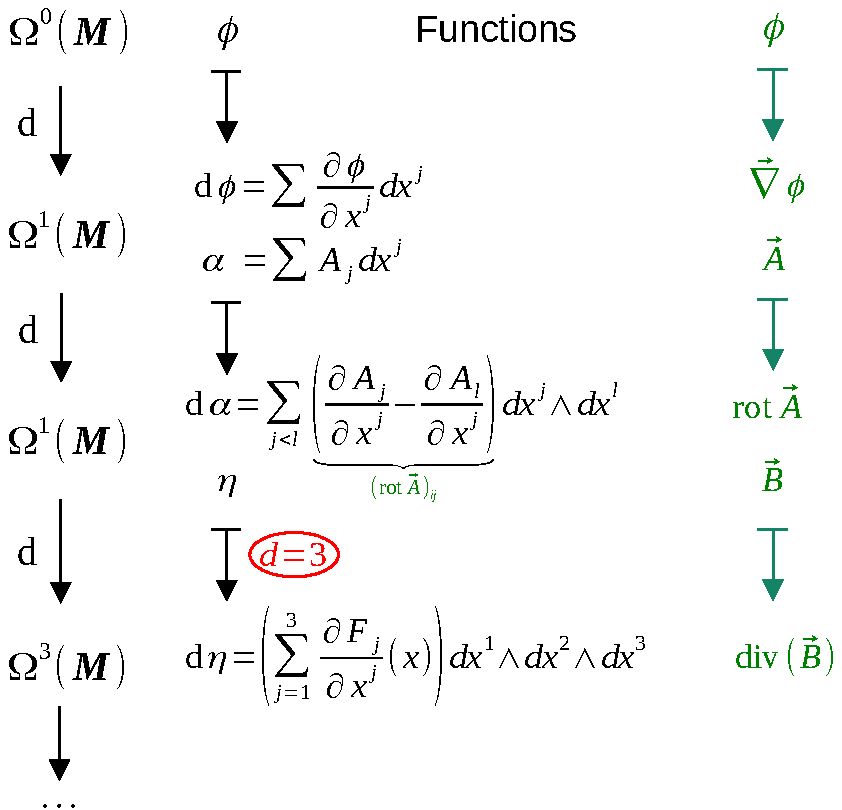
\includegraphics{images/schema_confronto_diff_analisi.pdf}
	\caption{Scheme of the comparison between differential forms and vector analysis. At some point the chain will stop, because on a manifold of dimension $n$ you can have differential forms up to degree $n$. As we have seen in \vrefch{diff_form_I}, dimension $3$ is somehow "special" since allows us to identify vector fields with 2-forms (instead, given a metric, the identification with 1-forms is always possible).}
	\labfig{schema-confronto-diff-analisi}
\end{figure}
The correspondence between differential forms and vector fields is not so innocent as the schetch in \reffig{schema-confronto-diff-analisi} may let us think. If we want to do it precisely and to write an isomorphism between spaces, we need to introduce a metric and use the so-called \href{https://en.wikipedia.org/wiki/Hodge_star_operator}{Hodge duality}, but since it is not so central for us, we will leave it as a starred exercise.\marginnote[-80mm]{The "\href{https://en.wikipedia.org/wiki/Curl_(mathematics)}{Curl}" should be denoted as "curl", but since the professor is habituated to the Italian notation, he denotes it as "div".}\\
{\fontencoding{U}\fontfamily{futs}\selectfont\char 66\relax} Message: Cartan differential \textbf{d} is a simultaneous generalisation of the operators of vector analysis ($\vec{\nabla}, \textrm{rot}, \textrm{div}, \dots$) and, with respect to that
\begin{enumerate}
    \item The universal property $\textrm{d}^2=0$ generalized
    \begin{enumerate}
        \item \(\ \ \textrm{rot}\ \vec{\nabla}\phi(x)=0 \qquad \textrm{d}\left(\textrm{d}\phi\right)=0\)
        \item \(\textrm{div}\ \textrm{rot}\vec{F}(x)=0 \qquad \textrm{d}\left(\textrm{d}\alpha\right)=0\)
    \end{enumerate}
    \item The \textbf{pseudo-Leibniz property}\index{Pseudo-Leibniz property} generalizes:
    \begin{enumerate}
        \item $\vec{\nabla}\left(\phi\psi\right)=\vec{\nabla}\phi\cdot\psi+\psi\vec{\nabla}\psi$
        \item \(\textrm{rot}\left(\varphi\vec{V}\right)=\vec{\nabla}\varphi\times\vec{V}+\varphi \ \textrm{rot}\vec{V}\)
        \item \(\textrm{div}\left(\varphi\vec{V}\right)=\vec{\nabla}\varphi\cdot\vec{V}+\varphi \ \textrm{div}\vec{V}\)
        \item \(\textrm{div}\left(\vec{X}\wedge\vec{Y}\right)=\textrm{rot}\vec{X}\cdot\vec{Y}\ {\color{red}\underset{\mathclap{\tikz \node {\color{red}$\uparrow$} node [below=1ex] {\footnotesize \color{red} \underline{minus!} };}}{-}}\ \vec{X}\cdot\vec{Y}\)
    \end{enumerate}
    everything with $\textrm{dim}\mathbf{M}=3$
\end{enumerate}
\section{\href{https://it.wikipedia.org/wiki/Henri_Poincar\%C3\%A9}{Poincaré} lemma and its converse}
\label{Poincaré}
In vector analysis we use to ask our self if a vector field is the gradient of some potential, and we know that this happens if the field is conservative\sidenote{the rotational curl vanishes} and the space is nice\sidenote{It is simply connected, like the full $\mathbb{R}^n$}. The same problems appears with the differential forms: we can ask our self if it happens that our differential form is the differential of a lower degree form, i.e. when it happens that a k-form is the Cartan differential of a (k-1)-form.
\begin{kaobox}[frametitle=Terminology]
A k-form $\omega\in\Omega^k(\mathbf{M})$ is \textbf{closed}\index{Closed k-form} if ${\color{red}\textrm{d}\omega=0}$.\\
A k-form $\omega\in\Omega^k(\mathbf{M})$ is \textbf{exact}\index{Exact k-form} if $\exists \ \alpha\in\Omega^{\color{red}k-i}(\mathbf{M})$ such that ${\color{red}\textrm{d}\alpha=\omega}$
\end{kaobox}
There is a result, historically known as Poincaré lemma, that for our viewpoint is trivial because he lived before the time of Cartan
\begin{lemma}[\href{https://it.wikipedia.org/wiki/Lemma_di_Poincar\%C3\%A9}{Poincaré lemma}]\index{Poincaré lemma}
Any \textbf{exact form is closed.}
\end{lemma}
\begin{proof}
If $\omega$ is exact, then $\omega = \textrm{d}\alpha$ for some $\alpha\in\Omega^{k-1}(\mathbf{M})$. Then $\textrm{d}\omega=\textrm{d}\left(\textrm{d}\alpha\right)=0$.
\end{proof}
What it is not obvious is the converse, that in general is false.\\
\underline{Problem:} Given a \textbf{\underline{closed}} $\omega\in\Omega^k(\mathbf{M})$, it is true that $\exists \ \alpha \in \Omega^{k-1}(\mathbf{M})$ such that $\textrm{d}\alpha=\omega$??\\
\underline{Answer:} In general \underline{\textbf{no!!}} There might be \textbf{topological obstruction} related to "holes" of $\mathbf{M}$.\marginnote[-35mm]{The fact that is closed, it is not sufficient to guarantee that the form is exact. This is the generalization (or the counterpart) of what happens in vector analysis: the fact that a vector field is irrational, does not always implies that is the gradient of some potential function, because you need the space to be simply connected (a loop must be continuously deformed to zero). The same happens for a divergence free vector field.}\\
But if you are in some nice manifold, then it works. Hence it does not only depend on the form (vector field), but it depends also and crucially on the structure of the manifold (it will not be the same to be in a sphere or a torus or something else). There are several examples of that:
\begin{marginfigure}[-10mm]
    \centering
	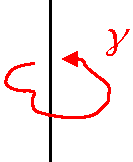
\includegraphics[width=0.5\linewidth]{images/ex1_topol_obstruction.pdf}
	\caption{Example one of topological obstruction}
	\labfig{ex-1-top-obs}
\end{marginfigure}
\begin{example}
$\boxed{k=1}\ $ If we are interested in 1-forms and we take the real 3D space minus an infinite wire $\mathbf{M}=\mathbb{R}^3\slash \left\{\left(0,0,2\right): z\in\mathbb{R}\right\}$. We see that this is not simply connected. There are some loops which are not continuously deformable to a point \textbf{in} $\mathbf{M}$, therefore \[\exists \ \alpha \in \Omega^1(\mathbf{M})\ \textrm{ one forms which is closed but \textbf{not exact}}\]
\end{example}
\begin{marginfigure}[-10mm]
    \centering
	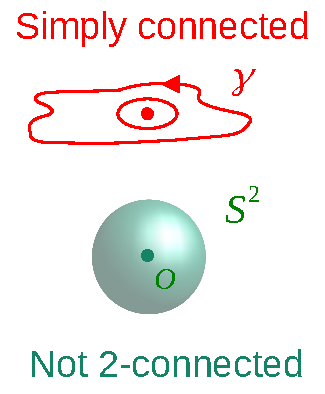
\includegraphics[width=0.6\linewidth]{images/ex2_topol_obstruction.pdf}
	\caption{Example one of topological obstruction.}
	\labfig{ex-2-top-obs}
\end{marginfigure}
\begin{example}
$\boxed{k=2}\ $ If we are interested in 2-forms and we take $\mathbf{M}=\mathbb{R}^3\slash \left\{\left(0,0,0\right)\right\}$. In this case every loop can be deformed to the trivial loop (it is simply connected), which is identical to a point, but is not 2-connected: it is not true that every 2-sphere can be continuously deformed to a point. Therefore
\[\exists \ \beta \in \Omega^2(\mathbf{M})\ \textrm{ one forms which is closed but \textbf{not exact}}\]
\end{example}
\underline{Details:} Book \sidecite{von1978differential} or \cite{doCarmo1994}.\\
The way-out from this problem is assuming that our manifold is good enough. Otherwise there could be some interesting effect, for example a magnetic field that does not admit a vector potential is interesting in itself. for some application is even more interesting than the ordinary case. Anyway, for very nice space the following proposition holds true
\begin{proposition}[Converse to Poincaré lemma]
Let $\mathbf{M}$ be a manifold. Suppose that $\mathbf{M}$ is \textbf{contractible}\footnote{$\mathbf{M}$ can be \textbf{continuously} deformed to a single point (ex: $\mathbf{M}=\mathbb{R}^d$).}. Then for any $\omega\in\Omega^k(\mathbf{M})$ we have the fact that
\[
\textrm{d}\omega=0 \ \underset{\mathclap{\tikz \node {$\uparrow$} node [below=1ex] {\footnotesize $\mathbf{M}$ contractible };}}{\Rightarrow} \ \exists \ \eta\in\Omega^{k-1}(\mathbf{M}) \ \textrm{ such that } \ \textrm{d}\eta = \omega
\]
\end{proposition}
This is a general result, if you are interested in 1-form or 2-forms, there are more specific results.
\section[Pull-back of differential forms]{\href{https://it.wikipedia.org/wiki/Pull-back}{Pull-back}\sidenote{"Regressione" in Italian, but also in Italian is used "Pull-back".} of differential forms}
Consider a smooth map and a differential form of degree $k$ on the target (arrival) space as in \reffig{pull-back}
\[
\mathbf{M}\xrightarrow[f]{C^\infty}\mathbf{N}, \quad \omega \in \Omega^k(\mathbf{N})
\]
\begin{figure}[H]
	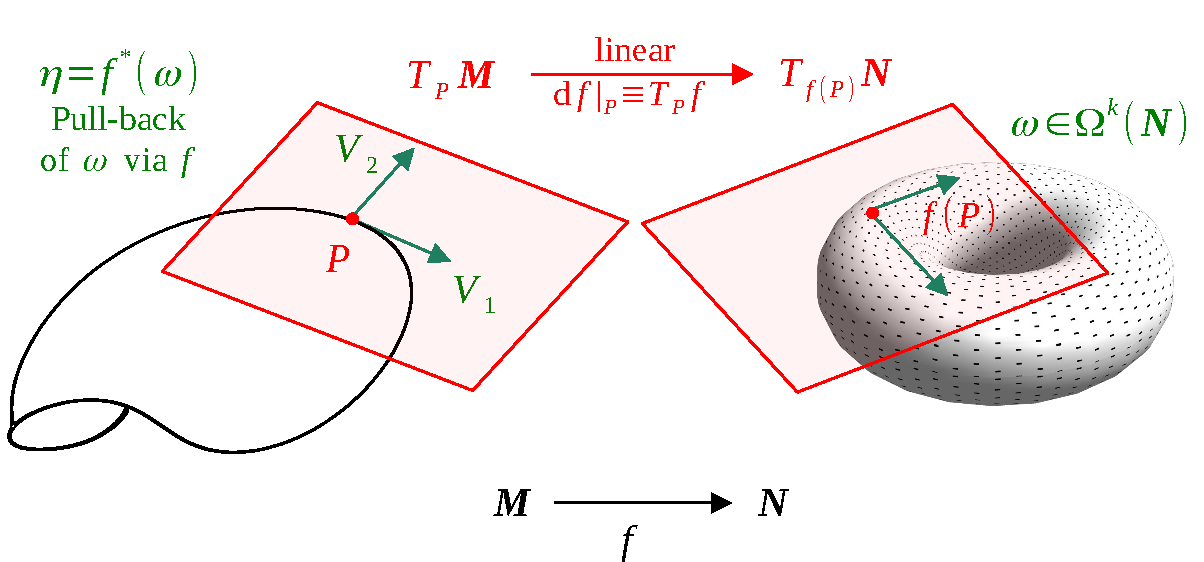
\includegraphics{images/pull_back.pdf}
	\caption{Pull-back of a differential form. The notation of the linear map changes accord to the book.}
	\labfig{pull-back}
\end{figure}
We want to construct a differential form $\eta$ of the same degree on manifold $\mathbf{M}$ of the source space, which will be obtain by $\omega$ by pulling it back\sidenote{"Tirandola indietro" in Italian. For this reason is called the "Pull-back" of $\omega \textrm{ via } f$.} We want to define the pull-back $f^\ast(\omega)_P$ in a natural way. We want it to produce a number when applied to vectors, and the only thing we have in our hands is $\omega$. There it should be related to in the only natural point $f(P)$ and the corresponding vectors in the tangent space on the arrival space. To relate them we can use the differential of a map, that maps every green vector in two green vectors on the arrival space. Therefore:
\[
{\color{red} f^\ast(\omega)_P}\left(V_1,\dots,V_k\right):= {\color{red}\omega_{f(P)}}\left({\color{red}\textrm{d}f_P}(V_1),\dots,{\color{red}\textrm{d}f_P}(V_K)\right)
\]
$\textrm{with } \ V_1,\dots,V_k \in T_P\mathbf{M}$. This "natural" definition provides a k-form $\eta\in\Omega^k(\mathbf{M})$ which is called the \textbf{pull-back of $\omega$ via $f$}\index{Pull-back of diff. forms}. We should check that this is a differential form, but this is boring, the only interesting part is to guess what is the natural and good definition. Why is this interesting to physicist? Because\\
{\fontencoding{U}\fontfamily{futs}\selectfont\char 66\relax} A change of variable on $\mathbf{M}$ is "naturally" expressed as a pull-back
\[
\mathbf{M}\xrightarrow[C^\infty]{f}\mathbf{M} \qquad \textrm{OLD}=f(\textrm{NEW})
\]
If $\omega\in\Omega^1(\mathbf{M})$ represents something (vector potential, magnetic field, simplectic form, etc..) in the OLD variables, then $f^\ast(\omega)\in\Omega^1(\mathbf{M})$ is the same (physical) thing in the new variables.\sidenote{Just remember that you have to put the new variables in the source space and not vice-versa.}
\begin{example}
(easy). Let 
\[
\omega = \frac{1}{x^2+y^2}\left(-ydx+xdy\right)
\]
be a 1-form in $\mathbb{R}^2 \setminus \left\{0\right\}$ equipped $(x,)=(x^1,x^2)$. Then we put a restricted to the circle
\[
\eta=\omega\Big|_{S^1}=-ydx+xdy
\]
Consider a map that goes around the circle
\[
\begin{split}
f:\mathbb{R}& \to \mathbb{R}^2\\
\theta &\mapsto \left(\cos\theta,\sin\theta\right)
\end{split}
\]
Compute explicitly the the pull-back of $f^\ast(\eta)$ and check its relation with the change of variable $(x,y)\ \longleftrightarrow \ \theta$.
\end{example}
Now that we know that the pull-back is a change of variable, it is important to know that the pull-back it is very well compatible with respect the operation on differential forms, namely the wedge product and the stereo differential. Otherwise it should arise the problem: "Should I first differentiate or first change variables?". The answer is that it does not matter.
\begin{proposition}
Given $\varphi:\mathbf{M}\to\mathbf{N}$, the pull-back satisfies the following properties:
\begin{enumerate}
    \item linear: $\varphi^\ast\left(\omega+\eta\right)=\varphi^\ast\left(\omega\right)+\varphi^\ast(\eta)$
    \item {\color{red}$\wedge$-compatible}:
    \(
    \varphi^\ast\left(\omega\wedge\eta\right)=\varphi^\ast(\omega)\wedge\varphi^\ast(\eta)
    \)
    \item {\color{red}d-compatible}: $\varphi^\ast(\textrm{d}\omega)=\textrm{d}\varphi^\ast(\omega)$
    \item composition-compatible: 
    \begin{tikzcd}
            \mathbf{M}\rar{\varphi}\arrow[black, bend right]{rr}[black,swap]{\psi\circ\varphi}  & \mathbf{N} \rar{\psi}  & \mathbf{Q}
    \end{tikzcd}
    \begin{equation}\labeq{comp-pull-back}
        \left(\psi\circ\varphi\right)^\ast(\omega)=\varphi^\ast\left(\psi^\ast\omega\right)
    \end{equation}
\end{enumerate}
\end{proposition}
Somebody could say "I could change variable step by step or once for all": i.e. given a $\omega$ form, if take the change of variable $\psi\circ\varphi$ and take the pull-back via this big change of variable, this is a change of variable only if $\mathbf{M}\cong\mathbf{N}\cong\mathbf{Q}$. Or we could do it step by step as in \refeq{comp-pull-back} and the big news is that they are equal. This is particular important for us physicist when we interpret pull-back as a change of variable, because it is telling us that the wedge product and the differential behave nicely with respect to change of variable.\sidenote{N.B. the same is not true for the differential operator of vector analysis. For example, try to take a rotor/curl in spherical coordinates, it will look something else. This is why the calculus with differential form is considered superior to the calculus we learned in \href{https://corsidilaurea.uniroma1.it/it/view-course-details/2021/30046/20210916103754/f3f180f6-5ec9-4154-815c-e2f83313823b/68f72759-7d11-41c3-a5c7-c41526bd695e/24308e39-e91d-4ec8-8fdb-00731a560baa/a0debc1a-f1c3-405d-82fe-967d44c7413a?guid_cv=68f72759-7d11-41c3-a5c7-c41526bd695e&current_erogata=f3f180f6-5ec9-4154-815c-e2f83313823b}{Vector Analysis (Analysis II)}.}
\section[Reformulation of electrodynamics with differential forms]{Reformulation of (classical) electrodynamics with differential forms}
The first application of this theory is the reformulation of classical electrodynamics in terms of differential forms.
\begin{marginfigure}
	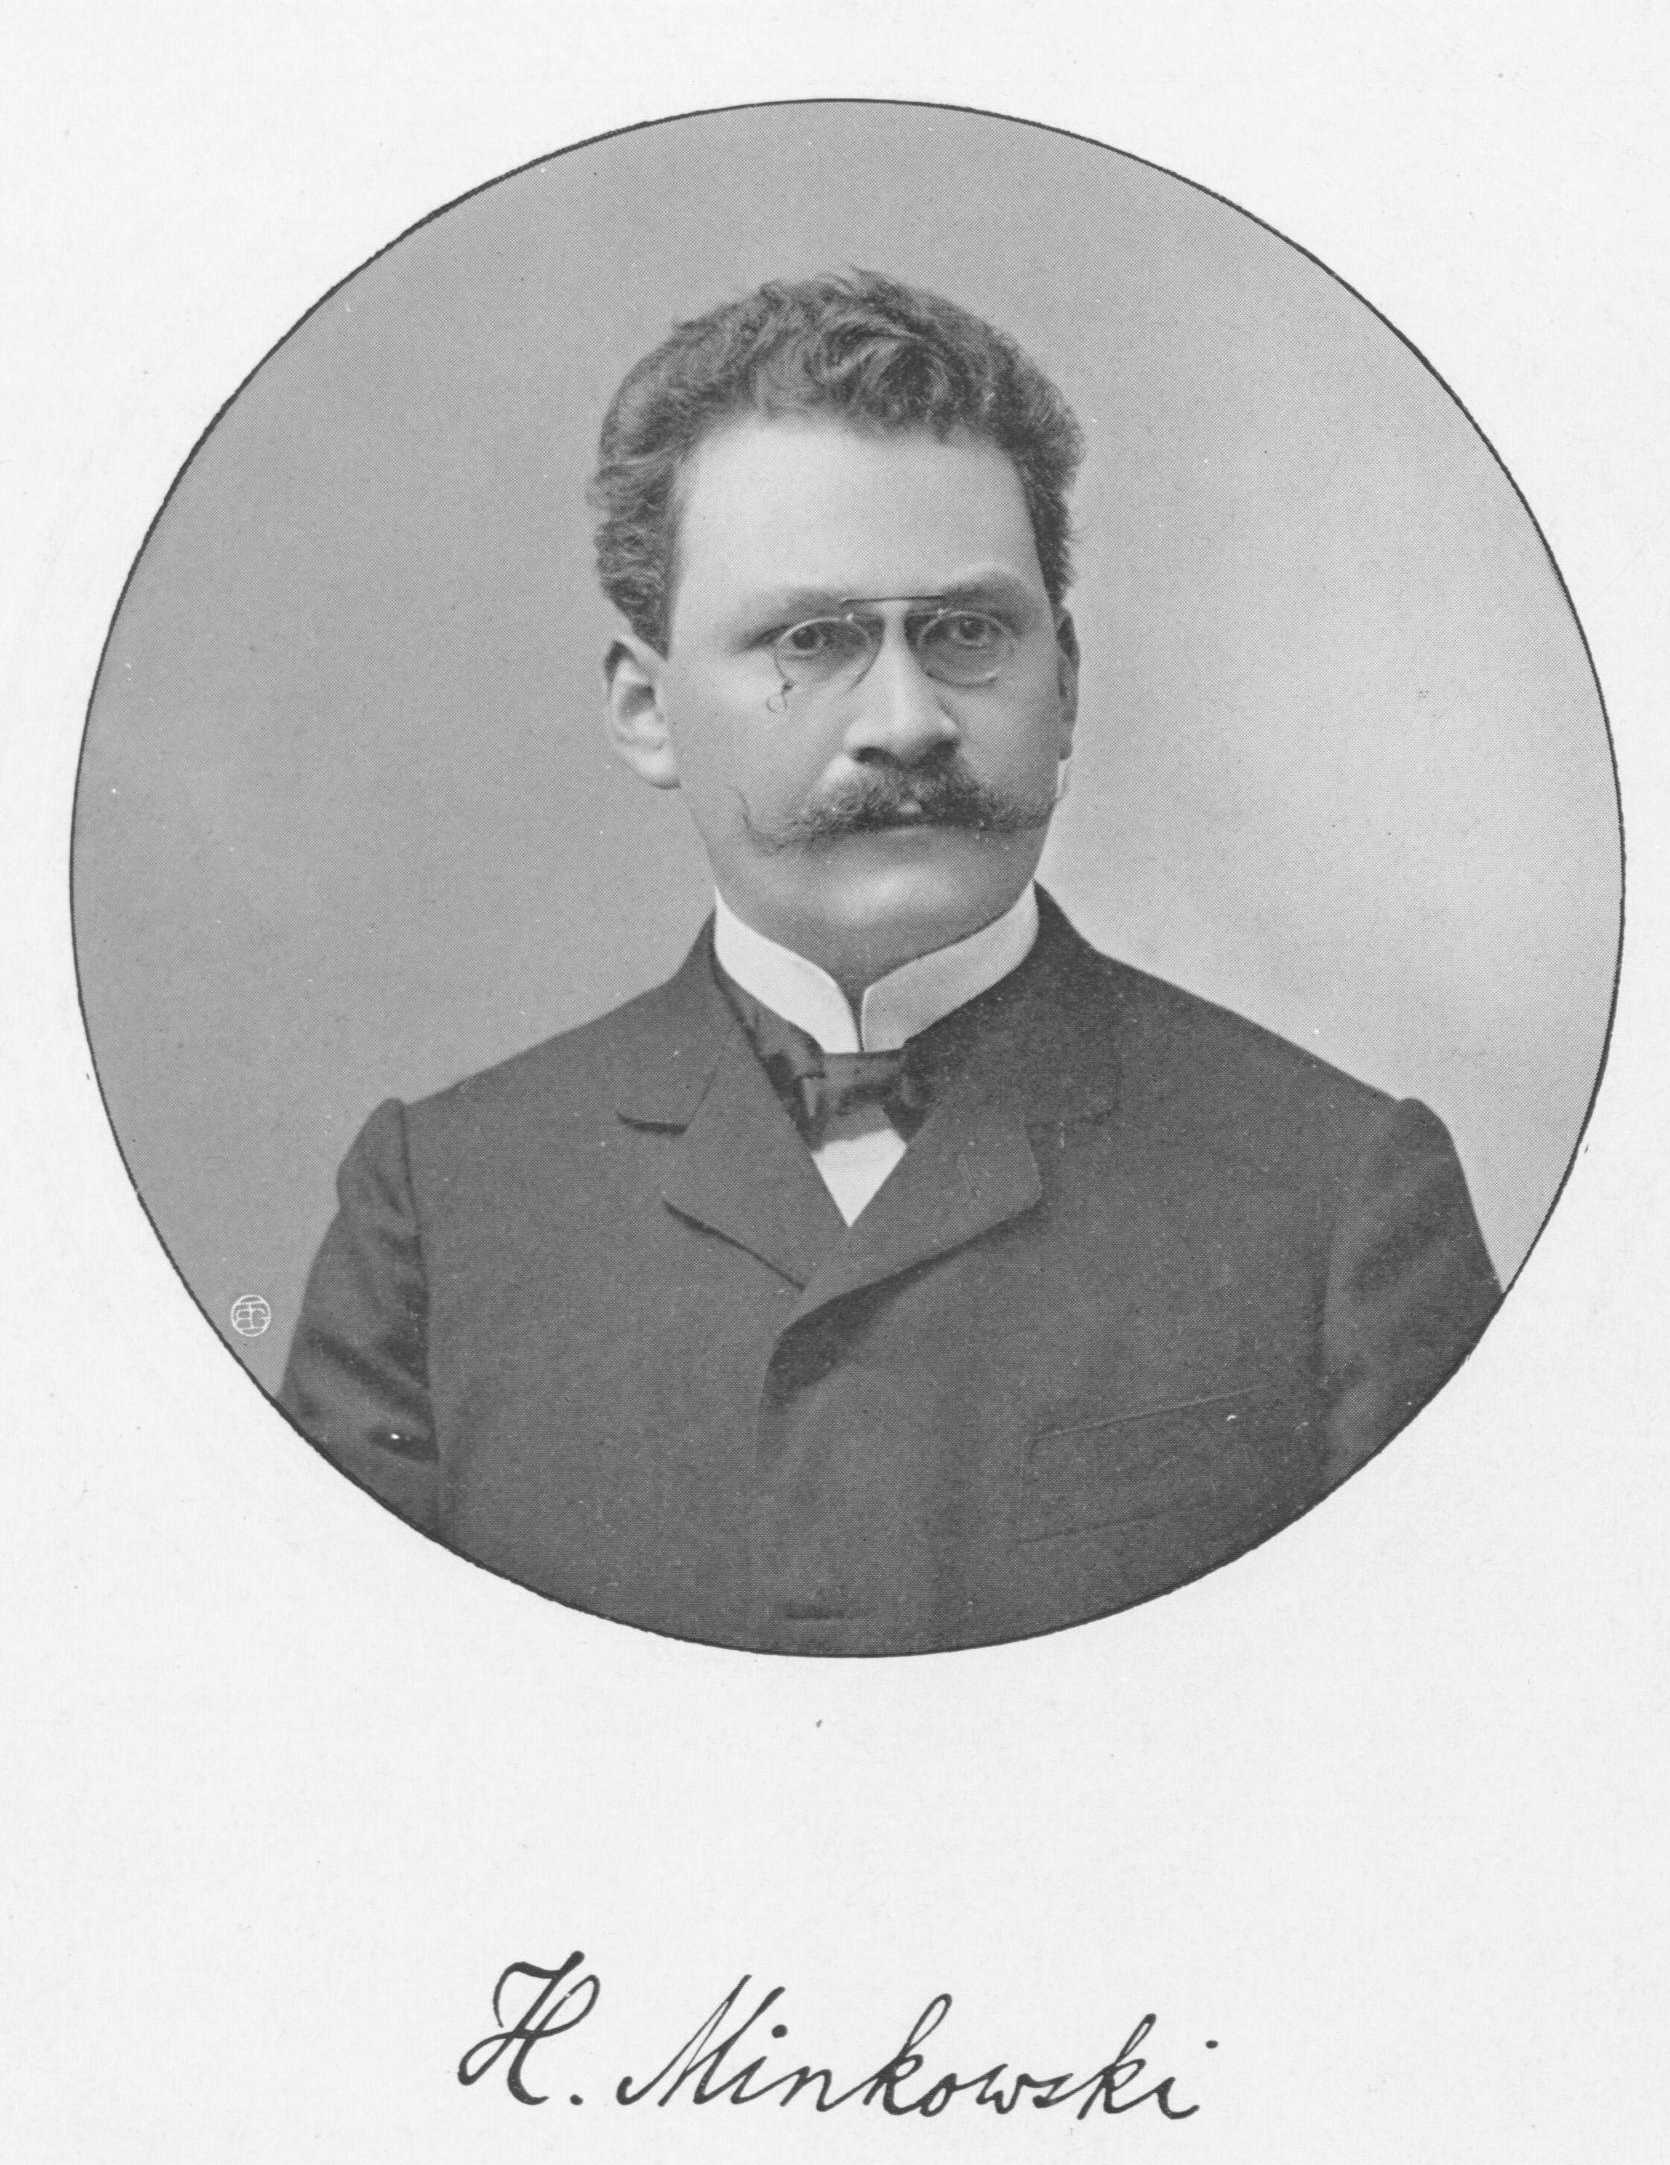
\includegraphics[width=1\linewidth]{images/De_Raum_zeit_Minkowski_Bild.jpg}
	\caption{From \href{https://commons.wikimedia.org/wiki/File:De_Raum_zeit_Minkowski_Bild.jpg}{Wikimedia}: Hermann Minkowski (1864-1909) found that the theory of special relativity, introduced by his former student Albert Einstein, could be best understood as a four-dimensional space, since known as the Minkowski spacetime.}
	\labfig{Minkowski}
\end{marginfigure}
\paragraph{\underline{Setting:}} We will consider a $\mathbf{M}$ manifold with {\color{red}$\textrm{dim}\mathbf{M}=4$} as space-time. To start with, we will be even more specific, we will consider the $\mathbb{M}$ \href{https://it.wikipedia.org/wiki/Spaziotempo_di_Minkowski}{Minkowski space}\sidenote{"spaziotempo di Minkowski" in Italian.}
, as know, regarded as a linear space over a manifold can be identified with $\mathbb{M}\cong\mathbb{M}^4$, which means it is a \underline{\textbf{flat}} manifold. This fact as two important consequences:
\begin{enumerate}
    \item there exist infinitely many global charts and coordinates, we will denote them with $\left(x^0,x^1,x^2,x^3\right)\equiv \left(x^0\vec{x}\right)$;
    \item there is a natural identification\sidenote{As always happens, if you have a linear space, the tangent to the linear space can be identify with the space itself, even though sometimes is convenient to distinguish the,} between the tangent space to the Minkowski at a point and the Minkowski space itself: $T_P\mathbb{M}=\mathbb{M}$.
\end{enumerate}
But the Minkowski space is not just $\mathbb{R}^4$, but is $\mathbb{R}^4$ equipped with:\index{Lorentzian metric}
\[
\textrm{\textbf{Lorentzian metric:} biliniear, symmetric, signature} \ (1,3)
\]
\[
\langle v,w\rangle_{\underset{\mathclap{\tikz \node {$\uparrow$} node [below=1ex] {\footnotesize metric};}}{g}}=\sum g_{\mu\nu}v^\mu w^\nu \quad \forall \ v,w \in T_P\mathbb{M}
\]
The signature can be
\[
\begin{split}
    \textrm{Positive signature:} \ (-,+,+,+)=(1,3) \quad & \textrm{used in General Relativity}\\
    \textrm{Negative signature:} \ (+,-,-,-)=(3,1) \quad & \textrm{used in High Energy Physics}
\end{split}
\]
according to the convection. The $g$ as subscript is to remind our self that it comes from a metric (bilinear and symmetric) and that it is not the inner product of a Hilbert space (sesquilinear and hermitian). As we heard several times, one of the basic principle of the theory is that an inertial frame, in the physical reality, corresponds to an inertial frame in our theory.
\[
\text{\parbox{4 cm}{\centering Inertial \\[-4pt] frame \\[-4pt] (structure)}}\longleftrightarrow\text{\parbox{4 cm}{\centering Lorentzian \\[-4pt] frame  \\[-4pt] (bases/chart)}}
\]
Notice that the word \textit{frame} is used with two different meanings on the two sides of the arrow:
\begin{itemize}
    \item \textbf{Physical reality}: inertial frame is a macroscopic rigid structure with three orthonormal axes and a clock. It is an inertial structure in the laboratory.
    \item \textbf{Mathematical reality}: Lorentian frame is a bases (or system of coordinates) which the special property that it can diagonlize the metric: in an inertial frame $\leftrightarrow$ Lorential frame if you take the vector of this special bases and the inner product you get
    \[
    \langle e_\mu, \e_\nu \rangle_g = g_{\mu\nu} \quad \longleftarrow \quad\pqty{g_{\mu\nu}}=\mqty(\dmat{1,-1,-1,-1})
    \]
    In particular, only in an inertial frame, the length of a vector is
    \[
    \norm{u}_g=\bqty{u^0}^2-\norm{\vec{u}}^2
    \]
\end{itemize}
%1:49:00
%FINE LEZIONE 7 24/03/2022
%INIZIO LEZIONE 8 25/03/2022
\section{Review of relativistic mechanics}
As we know, the Newton equations are not compatible with special relativity. Why? Because to compute accelerations we need to select a distinguish time axis and this is not compatible with the principle of special relativity. We have to replace the Newton equation with something else and the idea, due to Einstein itself, is based on the idea of proper time.
\subsection{Proper time}
We fix an inertial frame, or a Lorentzian chart, and we draw the \textbf{world line} of our particle.
\begin{marginfigure}
    \centering
	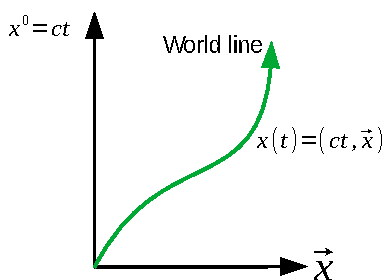
\includegraphics[width=1\linewidth]{images/World_line.pdf}
	\caption{Schematic representation of a world line.}
	\labfig{world_line}
\end{marginfigure}
Now we define the \textbf{proper time}, a sort of reparametrization of this path:  
\[
\tau(t)=\int_{t_0}^t dt'\sqrt{1-\frac{|\Vec{v}(t')|}{c^2}}
\]
Physically, this is the time given by a clock moving with the system, synchronized at time $t_0$ with the official clock of the inertial frame.
\subsection{Tetra-velocity}
Once we are equipped with the proper time, we can define the \textbf{tetra-velocity}
\[
u^{\mu}(\tau):=\frac{dx^{\mu}(\color{red}\tau)}{d\color{red}\tau}
\]
What is its relation with the ordinary velocity? It is given by the chain rule:
\[
u^{\mu}=\frac{dx^{\mu}}{d\tau}=\frac{dx^{\mu}}{dt}\frac{dt}{d\tau}=\frac{dx^{\mu}}{dt}\frac{1}{d\tau/dt}=\frac{1}{\sqrt{1-\frac{v(t)^2}{c^2}}}{\color{red}\frac{dx^{\mu}(\tau(t))}{\underset{\mathclap{\tikz \node {$\uparrow$} node [below=1ex] {\footnotesize ordinary velocity };}}dt}}
\]
What is remarkable is that the Lorentzian norm of the tetra-velocity is constant: $\rVert u \rVert^2_g=\langle u,u \rangle_g=c^2$. Suppose to have a particle at rest in the point $x_0$ which stays at rest forever: the world line will be equal to $(ct,\Vec{x_0})$, with tetra-velocity $(c,\Vec{0})$. This holds true for any other curve.\marginnote{The check of this relation is left as an exercise.}
\subsection{Tetra-acceleration}
We go on and we define the \textbf{tetra-acceleration}:
\[
a^{\mu}(\tau):=\frac{du^{\mu}(\color{red}\tau)}{d\color{red}\tau}
\]
The tetra-velocity has a peculiar geometric relation with the tetra-acceleration, they are \textbf{Lorentz orthogonal}:
\[
0=\frac{d}{d\tau}\langle u,u \rangle_g\underset{\mathclap{\tikz \node {$\uparrow$} node [below=1ex] {\footnotesize Leibnitz };}}=\langle\frac{d}{d\tau}u,u\rangle_g+\langle u,\frac{d}{d\tau}u\rangle_g\underset{\mathclap{\tikz \node {$\uparrow$} node [below=1ex] {\footnotesize symmetric};}}=2\langle u,\frac{d}{d\tau}u\rangle_g=2\langle u,a \rangle_g
\]
it means that for any world line, i.e. any possible cinematic, ${\color{red}\langle u,a \rangle_g=0}$, so geometrically it means they are orthogonal but with respect to the Lorentzian metric: ${\color{red}u(\tau)\perp_g a(\tau)}$
\subsection{Relativistic version of Newton equation}
We are now ready to write the relativistic version of the Newton equation:
\[
\star \Big|\Big| \quad m\frac{d}{d\tau}u^{\mu}(\tau)=\underbrace{f(x(\tau),u(\tau))}_{\textrm{tetra-force\marginnote{We sill have to understand the relation between the tetra-force and the force in three dimensional space.}}}
\]
Not every vector field on the Minkowski space is admissible as a tetra-force, because there is a constraint between the 0-component and the space-components.
The \textbf{orthogonality relation} ${\color{red}a\perp_g u}$ implies that\\
$f\perp_g u$, hence the 4-components of the tetra-force $f=(f^0,\vec{f})$ are \underline{\textbf{not}} \textbf{independent}:
\[
0=\langle u,f \rangle_g=cf^0-\vec{v}\cdot\vec{f}\Rightarrow f^0(x,\underset{\mathclap{\tikz \node {$\uparrow$} node [below=1ex] {\footnotesize $(u^0,\vec{v})$};}}u)=\frac{1}{c}\vec{f}\cdot\vec{v}
\]
Explicitly, in an inertial frame, RNE\sidenote{RNE=Relativistic Newton Equation} reads as follows:
\[
\begin{cases}
\frac{d}{dt}\frac{mc}{\sqrt{1-v^2/c^2}}=\sqrt{1-\frac{v^2}{c^2}}f^0\Rightarrow \frac{d}{dt}\underbrace{\frac{mc^{\color{red}2}}{\sqrt{1-v^2/c^2}}}_{\mathclap{\text{relativistic kinetic energy\marginnote{$E_{kin}\simeq mc^2+\frac{1}{2}mv^2+\mathcal{O}(v/c)$ as $v/c\xrightarrow[]{}0$}}}}=\sqrt{1-\frac{v^2}{c^2}}{\color{red}\vec{f}\cdot\vec{v}}=\vec{F}\cdot\vec{v}\xleftarrow[]{}\text{power of $\vec{F}$} \\
\frac{d}{dt}\frac{m\vec{v}}{\sqrt{1-v^2/c^2}}=\sqrt{1-\frac{v^2}{c^2}}\vec{f}=:\vec{F}\xleftarrow[]{}\text{force field in an inertial frame}
\end{cases}
\]
\section{Determination of tetra-force}
We now want to decide which kind of vector fields are admissible as a tetra-force, in particular which one corresponds to the usual Lorentz force of electrodynamics.\\
\underline{Problem:} characterize tetra-forces such that $\langle f(x,u),u \rangle_g=0$.\\
$\triangleright$ We suppose that $f(x,u)$ \textbf{depends linearly} on $u$. From the physical viewpoint, we know that the Lorentz force is linear in the velocity and from the mathematical viewpoint, we remember that if a force field is more than linear in the velocity (i.e. quadratic, depends on $u^{3/2}$) then it is not compatible with the Lagrangian formalism. This means that
\[
f^{\mu}(x,u)=\sum_{\nu}\Tilde{F}_{\nu}^{\mu}(x)u^{\nu}
\]
$\triangleright$ We impose the constraint $\langle f(x,u),u \rangle_g=0$:
\[
\sum_{\sigma,\nu,\mu}u^{\sigma}\underbrace{g_{\sigma\mu}\Tilde{F}_{\nu}^{\mu}}_{\color{red}=:\Tilde{F}_{\sigma\nu}}=\sum_{\sigma\nu}u^{\sigma}\Tilde{F}_{\sigma\nu}u^{\nu}=0 \quad \forall u\in T\mathbb{M}
\]
This implies that $\Tilde{F}$ is \textbf{anti-symmetric}: ${\color{red}\Tilde{F}_{\sigma\nu}=-\Tilde{F}_{\nu\sigma}}$
\[
\sum_{\color{red}\sigma<\nu}u^{\sigma}u^{\nu}\Tilde{F}_{\sigma\nu}(x) + \sum_{\color{red}\nu<\sigma}u^{\sigma}u^{\nu}\Tilde{F}_{\sigma\nu}(x) = \sum_{\color{red}\sigma<\nu}u^{\sigma}u^{\nu}\Tilde{F}_{\sigma\nu}(x) + \sum_{\color{red}\sigma^{'}<\nu^{'}}u^{\nu^{'}}u^{\sigma^{'}}\Tilde{F}_{\nu^{'}\sigma^{'}}(x)=
\]
\[
=\sum_{\sigma<\nu}u^{\sigma}u^{\nu}[\Tilde{F}_{\sigma\nu}(x)+\Tilde{F}_{\nu\sigma}(x)]=0\Rightarrow{\color{red}\Tilde{F}_{\sigma\nu}=-\Tilde{F}_{\nu\sigma}}
\]
An admissible tetra-force correspond to an \textbf{anti-symmetric, 2-covariant tensor field}, i.e. a \textbf{differential 2-form}
\[
\Tilde{\mathcal{F}}=\sum_{\mu<\nu}\Tilde{F}_{\mu\nu}(x)dx^{\mu}\wedge dx^{\nu}
\]
$\triangleright$ Now we add a piece of physical information: we know that in an inertial frame, the force field $\vec{F}$ is given by the \textbf{Lorentz force}:
\[
q\left[\vec{E}(x)+\frac{1}{c}\vec{v}\wedge\vec{B}(x)\right]^{\color{red}l}=\sqrt{1-\frac{v^2}{c^2}}\sum_{\nu=0}^3 \Tilde{F}_{\nu}^{{\color{red}\overset{\mathclap{\tikz \node {$\downarrow$} node [above=1.25ex] {\footnotesize space component};}}l}}(x)u^{\nu} \quad\text{for every } l\in\{1,2,3\} \quad (\star)
\]
$\triangleright$ As an exercise, one checks that $(\star)$ holds true if and only if\\  $\Tilde{F}_{\mu\nu}(x)=\frac{q}{c}F_{\mu\nu}(x)$
\[
F_{\mu\nu}=\begin{pmatrix}
0 & -E_x & -E_y & -E_z \\
E_x & 0 & B_z & -B_y \\
E_y & -B_z & 0 & B_x \\
E_z & B_y & -B_x & 0
\end{pmatrix}\marginnote{The signs depend on all the other conventions, so maybe if you change book you will have something else.}
\]
This is the 2-tensor which represents the electromagnetic field, also called the \href{https://en.wikipedia.org/wiki/Michael_Faraday}{Faraday} tensor.\sidenote{Although Faraday didn't know anything about 2-forms.}\\
\underline{Conclusion:} The electromagnetic field is described in an inertial/Lorentzian frame by the \textbf{2-form $\mathcal{F}$}$\in\Omega^2(\mathbb{M})$.
\[
\star \Big| \Big| \quad \Tilde{\mathcal{F}}=\sum_{\mu<\nu}\Tilde{F}_{\mu\nu}(x)dx^{\mu}\wedge dx^{\nu}
\]
Now we have written the force field as a differential 2-form, which is intrinsic so it does not depend on the change of coordinates even if we leave the clean world of Lorentzian frames. By the invariance of 2-forms under general change of coordinates, the last formula $\star$ describes the electromagnetic field in \textbf{any system of coordinates (or local chart)}.

\section{Maxwell equations}

\begin{align*}
  \begin{aligned}
    \text{div}\vec{B} &=0 & \text{rot}\vec{E} &=-\frac{1}{c}\frac{\partial\vec{B}}{\partial t} & \small{\text{homogeneous}}\marginnote{We write the equations using Gauss units. $\rho(x)$ is the charge density, $\vec{J}(x)$ is the current density and $x=(ct,\vec{x})$}\\
    \text{div}\vec{E} &=4\pi\rho &
    \text{rot}\vec{B} &=\frac{1}{c}\frac{\partial\vec{E}}{\partial t}+\frac{4\pi}{c}\vec{J} & \small{\text{inhomogeneous}}\\
    & \hspace{-1.85em}\small{\text{constraints}} & & \hspace{-1.75em}\small{\text{dynamical equations}}
  \end{aligned}
\end{align*}
The \textbf{homogeneous} equations are linear partial differential equations with no external terms, i.e. no sources, while the \textbf{inhomogeneous} equations instead contain the sources and they give us information about the relation with the distribution of charge and currents in the system. Sometimes, it is also convenient to read them by columns: the \textbf{dynamical equations} tell us how the fields evolve and the \textbf{constraints} state which conditions the vector fields have to satisfy at every time.\\
We are going to proceed by row. Suppose we are in the stationary case, i.e. no time derivative, and let's look at the \textbf{homogeneous} equation: they are both \textbf{conditions of closureness} of differential forms
\[
d\beta=0 \text{ with } \beta=\sum_{i,j=1}^3\mathbb{B}(x)_{ij}dx^i\wedge dx^j \quad d\eta=0 \text{ with } \eta=\sum_{i=1}^3 E_i(x)dx^i
\]
$\beta$ is builded up by the $3\times3$ part of the Faraday tensor while $\eta$ is builded up with the rows\marginnote{Or the columns, it is up to a sign and it depends on the convention used.} of the Faraday tensor.
\begin{proposition}
The \textbf{homogeneous Maxwell equations}, which are written in an inertial frame, are equivalent to the intrinsic equation $d\mathcal{F}=0$ where $\mathcal{F}=\sum F_{\mu\nu}(x)dx^{\mu}\wedge dx^{\nu}$ is the Faraday tensor. In components:
\[
\partial_{\rho}F_{\mu\nu}+\partial_{\nu}F_{\rho\mu}+\partial_{\mu}F_{\nu\rho}=0\marginnote{Some people refer to it as Bianchi identity but we are not sure this is historically accurate}
\]
where $\partial_{\rho}=\frac{\partial}{\partial x^{\rho}}$ and $(x^0,x^1,x^2,x^3)$ are local coordinates, not necessarily Lorentzian coordinates.
\end{proposition}
\begin{proof}
\begin{align*}
d\mathcal{F}&=\sum_{\mu<\nu}(dF_{\mu\nu}(x))\wedge dx^{\mu}\wedge dx^{\nu}=\sum_{\mu<\nu}\sum_{\lambda}\frac{\partial F_{\mu\nu}}{\partial x^{\lambda}}dx^{\lambda}\wedge dx^{\mu}\wedge dx^{\nu}=\marginnote{The indices $\mu,\nu,\lambda$ are not well ordered, so we regroup them. $\lambda$ cannot be equal to $\mu$ or $\nu$ otherwise we will have zero. Each permutation brings a minus sign.}\\
&=\sum_{{\color{red}\lambda}<\mu<\nu}\frac{\partial F_{\mu\nu}}{\partial x^{\lambda}}dx^{\lambda}\wedge dx^{\mu}\wedge dx^{\nu}+\\
&+{\color{red}(-1)}\sum_{\mu<\nu<{\color{red}\lambda}}\frac{\partial F_{\mu\nu}}{\partial x^{\lambda}}dx^{\mu}\wedge {\color{red}dx^{\lambda}}\wedge dx^{\nu}+\\
&+{\color{red}(-1)^2}\sum_{\mu<\nu<{\color{red}\lambda}}\frac{\partial F_{\mu\nu}}{\partial x^{\lambda}}dx^{\mu}\wedge dx^{\nu}\wedge {\color{red}dx^{\lambda}}=\\
&=\marginnote{We re-label the indices.}\sum_{{\color{red}\lambda<\mu<nu}}\left(\frac{\partial F_{\mu\nu}}{\partial x^{\lambda}}{\color{red}-}\frac{\partial F_{\lambda\nu}}{\partial x^{\mu}}+\frac{\partial F_{\lambda\mu}}{\partial x^{\nu}}\right)dx^{\lambda}\wedge dx^{\mu}\wedge dx^{\nu}=\\
&=\marginnote{We exchange the indices $\lambda$ and $\nu$ in the second term to produce a minus.}\sum_{\lambda<\mu<nu}\left(\frac{\partial F_{\mu\nu}}{\partial x^{\lambda}}{\color{red}+}\frac{\partial F_{\nu\lambda}}{\partial x^{\mu}}+\frac{\partial F_{\lambda\mu}}{\partial x^{\nu}}\right)dx^{\lambda}\wedge dx^{\mu}\wedge dx^{\nu}
\end{align*}
\end{proof}
We have now a powerful tool, which is the theory of differential forms, which allows us to prove in one line the existence of electromagnetic potential:
\begin{proposition}
There exists a 1-form $\alpha=\sum_{\mu=0}^3A_{\mu}(x)dx^{\mu}$ such that {\color{red}$d\alpha=\mathcal{F}$} i.e. {\color{red}$F_{\mu\nu}=\partial_{\mu}A_{\nu}(x)-\partial_{\nu}A_{\mu}(x)$}
\end{proposition}
\begin{proof}
Observe that $\mathbb{M}\cong\mathbb{R}^4$ is contractible, which means it can be continuously deformed to a point. By the converse of the Poincaré lemma [\ref{Poincaré}], {\color{red}$d\mathcal{F}=0$ (Maxwell equations)}.\\ $\exists\alpha\in\Omega^1(\mathbb{M}$ such that $d\alpha=\mathcal{F}$.
\end{proof}
We explicitly compute it now: the covariant components of the potential are
\[
A_0=V \, A_1=-A_x \, A_2=-A_y \, A_3=-A_z
\]
The corresponding \textbf{vector field} is {\color{red}$A^{\mu}=g^{\mu\nu}A_{\nu}$} where $g^{\mu\nu}=(G^{-1})^{\mu\nu}$\marginnote{If the ordinary metric is $g_{\mu\nu}=G$, then when we go to the indices upstairs, we should take the inverse matrix. In the Lorentzian metric, $G=G^{-1}$}:
\[
A^0=V \, A^1=A_x \, A^2=A_y \, A^3=A_z
\]
What is the message to take home? Any tetra-form has a relation between the 0-component and the spatial components and to be admissible it has to be given by a 2-covariant anti-symmetric tensor field which is a differential 2-form. If we insert a bit of physical information we get the Faraday tensor. Once we write it as a differential form, this holds true in any coordinate system.\\
How about the \textbf{inhomogeneous} Maxwell equation? Unlike the homogeneous ones, they are partially geometrical but that is because they involve the sources and there is no reason why they should be geometrical. The sources are completely described by a contravariant vector called the \textbf{tetra-current}:
\[
J^{\mu}(x)=(c\rho(t,\vec{x}),\vec{J}(t,\vec{x}))
\]
The \underline{\textbf{continuity equation}} which expresses the fact that the charge is locally conserved and in this formalism it can be written as:
\[
\sum_{\mu=0}^3\partial_{\mu}J^{\mu}(x)=0
\]
We want \textbf{I order PDEs\sidenote{PDE=Partial Differential Equation}} which involve a datum $J^{\mu}(x)$, which is contravariant, and either $F_{\mu\nu}$ or one of its "relatives" ($F_{\mu}^{\nu},F^{\mu\nu},\dots$). There are not many possibilities to satisfy this:
\[
\sum_{\nu=0}^3\partial_{\nu}F^{\mu\nu}=\frac{4\pi}{c}J^{\mu} \quad \Big| \Big| \,\small{\text{Inhomogeneous Maxwell equations}}
\]
where $F^{\mu\nu}=g^{\mu\sigma}g^{\nu\rho}F_{\sigma\rho}$. If we consider the \textbf{Minkowski metric} the corresponding matrix is diagonal:
\[
g^{\mu\nu}=g^{\mu\mu}\delta^{\mu\nu} \quad F^{\mu\nu}=g^{\mu\nu}g^{\nu\nu}F_{\mu\nu}
\]
The Faraday tensor now becomes:
\[
F^{\mu\nu}=\begin{pmatrix}
0 & E_x & E_y & E_z \\
-E_x & 0 & B_z & -B_y \\
-E_y & -B_z & 0 & B_x \\
-E_z & B_y & -B_x & 0
\end{pmatrix}
\text{ with } \mu,\nu\in\{1,2,3\}
\]
\end{document}